\let\negmedspace\undefined
\let\negthickspace\undefined
\documentclass[journal]{IEEEtran}
\usepackage[a5paper, margin=10mm, onecolumn]{geometry}
%\usepackage{lmodern} % Ensure lmodern is loaded for pdflatex
\usepackage{tfrupee} % Include tfrupee package

\setlength{\headheight}{1cm} % Set the height of the header box
\setlength{\headsep}{0mm}     % Set the distance between the header box and the top of the text

\usepackage{gvv-book}
\usepackage{gvv}
\usepackage{cite}
\usepackage{amsmath,amssymb,amsfonts,amsthm}
\usepackage{algorithmic}
\usepackage{graphicx}
\usepackage{textcomp}
\usepackage{xcolor}
\usepackage{txfonts}
\usepackage{listings}
\usepackage{enumitem}
\usepackage{mathtools}
\usepackage{gensymb}
\usepackage{comment}
%\usepackage{multiclo}
\usepackage[breaklinks=true]{hyperref}
\usepackage{tkz-euclide} 
\usepackage{listings}
% \usepackage{gvv} 
\graphicspath{ {./figs/} }

\begin{document}

\title{
ME: MECHANICAL ENGINEERING}
\author{AI25BTECH11011}
\maketitle
\renewcommand{\thefigure}{\theenumi}
\renewcommand{\thetable}{\theenumi}

\textbf{Q.1 - Q.5 carry one mark each.}
\begin{enumerate}

\item John Thomas, an ---------- writer, passed away in 2018.
\begin{multicols}{2}
\begin{enumerate}
    \item imminent
    \item prominent
    \item eminent
    \item dominant
\end{enumerate}
\end{multicols}
\hfill (GATE ME 2019)

\item ---------- I permitted him to leave, I wouldn't have had any problem with him being absent, ---------- I?
\begin{multicols}{2}
\begin{enumerate}
    \item Had, wouldn't
    \item Have, would
    \item Had, would
    \item Have, wouldn't
\end{enumerate}
\end{multicols}
\hfill (GATE ME 2019)

\item A worker noticed that the hour hand on the factory clock had moved by 225 degrees during her stay at the factory. For how long did she stay in the factory?
\begin{multicols}{2}
\begin{enumerate}
    \item 3.75 hours
    \item 4 hours and 15 mins
    \item 8.5 hours
    \item 7.5 hours
\end{enumerate}
\end{multicols}
\hfill (GATE ME 2019)

\item The sum and product of two integers are 26 and 165 respectively. The difference between these two integers is ----------.
\begin{multicols}{4}
\begin{enumerate}
    \item 2
    \item 3
    \item 4
    \item 6
\end{enumerate}
\end{multicols}
\hfill (GATE ME 2019)

\item The minister avoided any mention of the issue of women's reservation in the private sector. He was accused of ---------- the issue.
\begin{multicols}{2}
\begin{enumerate}
    \item collaring
    \item skirting
    \item tying
    \item belting
\end{enumerate}
\end{multicols}
\hfill (GATE ME 2019)

\textbf{Q. 6 – Q. 10 carry two marks each.}

\item Under a certain legal system, prisoners are allowed to make one statement. If their statement turns out to be true then they are hanged. If the statement turns out to be false then they are shot. One prisoner made a statement and the judge had no option but to set him free. Which one of the following could be that statement?
\begin{enumerate}
    \item I did not commit the crime
    \item I committed the crime
    \item I will be shot
    \item You committed the crime
\end{enumerate}
\hfill (GATE ME 2019)

\item A person divided an amount of Rs. 100,000 into two parts and invested in two different schemes. In one he got 10\% profit and in the other he got 12\%. If the profit percentages are interchanged with these investments he would have got Rs.120 less. Find the ratio between his investments in the two schemes.
\begin{multicols}{4}
\begin{enumerate}
    \item 9 : 16
    \item 11 : 14
    \item 37 : 63
    \item 47 : 53
\end{enumerate}
\end{multicols}
\hfill (GATE ME 2019)

\item Congo was named by Europeans. Congo's dictator Mobuto later changed the name of the country and the river to Zaire with the objective of Africanising names of persons and spaces. However, the name Zaire was a Portuguese alteration of Nzadi o Nzere, a local African term meaning 'River that swallows Rivers'. Zaire was the Portuguese name for the Congo river in the 16th and 17th centuries.

Which one of the following statements can be inferred from the paragraph above?
\begin{enumerate}
    \item Mobuto was not entirely successful in Africanising the name of his country
    \item The term Nzadi o Nzere was of Portuguese origin
    \item Mobuto's desire to Africanise names was prevented by the Portuguese
    \item As a dictator Mobuto ordered the Portuguese to alter the name of the river to Zaire
\end{enumerate}
\hfill (GATE ME 2019)

\item A firm hires employees at five different skill levels P, Q, R, S, T. The shares of employment at these skill levels of total employment in 2010 is given in the pie chart as shown. There were a total of 600 employees in 2010 and the total employment increased by 15\% from 2010 to 2016. The total employment at skill levels P, Q and R remained unchanged during this period. If the employment at skill level S increased by 40\% from 2010 to 2016, how many employees were there at skill level T in 2016?

\begin{figure}[H]
\centering
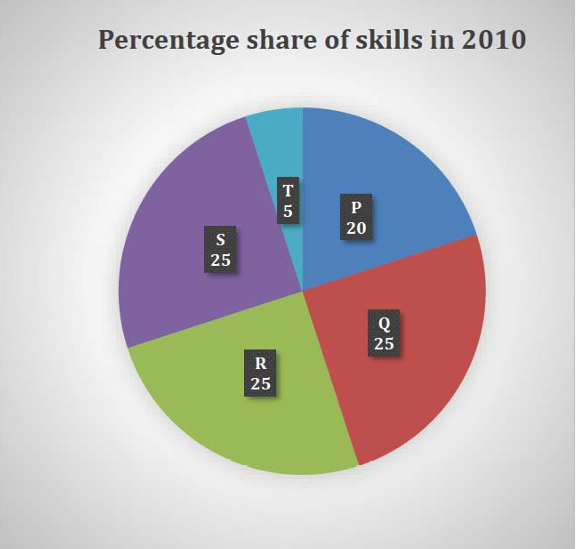
\includegraphics[width=0.4\textwidth]{Fig 1.png}
\caption{Percentage share of skills in 2010}
\label{fig:question9}
\end{figure}

\begin{multicols}{4}
\begin{enumerate}
    \item 30
    \item 35
    \item 60
    \item 72
\end{enumerate}
\end{multicols}
\hfill (GATE ME 2019)


\item M and N had four children P, Q, R and S. Of them, only P and R were married. They had children X and Y respectively. If Y is a legitimate child of W, which one of the following statements is necessarily FALSE?
\begin{enumerate}
    \item M is the grandmother of Y
    \item R is the father of Y
    \item W is the wife of R
    \item W is the wife of P
\end{enumerate}
\hfill (GATE ME 2019)

\end{enumerate}

\textbf{Q. 1 – Q. 25 carry one mark each.}

\begin{enumerate}
\item Consider the matrix
$\vec{P} = \myvec{1 & 1 & 0 \\
                  0 & 1 & 1 \\
                  0 & 0 & 1} $
The number of distinct eigenvalues of $ P $ is
\begin{multicols}{4}
\begin{enumerate}
    \item 0
    \item 1
    \item 2
    \item 3
\end{enumerate}
\end{multicols}
\hfill (GATE ME 2019)

\item A parabola $ x = y^2 $ with $ 0 \leq x \leq 1 $ is shown in the figure. The volume of the solid of rotation obtained by rotating the shaded area by 360° around the $ x $-axis is

\begin{figure}[H]
\centering
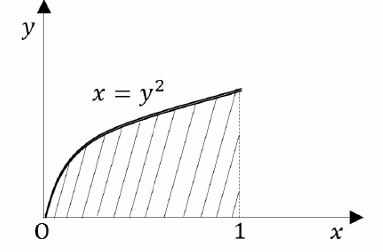
\includegraphics[width=0.5\textwidth]{Fig 2.png}
\caption{}
\label{fig:question2}
\end{figure}

\begin{multicols}{2}
\begin{enumerate}
    \item $\frac{\pi}{4}$
    \item $\frac{\pi}{2}$
    \item $\pi$
    \item $2\pi$
\end{enumerate}
\end{multicols}
\hfill (GATE ME 2019)

\item For the equation $\frac{dy}{dx} + 7x^2y = 0$, if $ y(0) = 3/7 $, then the value of $ y(1) $ is
\begin{multicols}{2}
\begin{enumerate}
    \item $\frac{7}{3} e^{-7/3}$
    \item $\frac{7}{3} e^{-3/7}$
    \item $\frac{3}{7} e^{-7/3}$
    \item $\frac{3}{7} e^{-3/7}$
\end{enumerate}
\end{multicols}
\hfill (GATE ME 2019)

\item The lengths of a large stock of titanium rods follow a normal distribution with a mean ($\mu$) of 440 mm and a standard deviation ($\sigma$) of 1 mm. What is the percentage of rods whose lengths lie between 438 mm and 441 mm?
\begin{multicols}{4}
\begin{enumerate}
    \item 81.85\%
    \item 68.4\%
    \item 99.75\%
    \item 86.64\%
\end{enumerate}
\end{multicols}
\hfill (GATE ME 2019)

\item A flat-faced follower is driven using a circular eccentric cam rotating at a constant angular velocity $ \omega $. At time $ t = 0 $, the vertical position of the follower is $ y(0) = 0 $, and the system is in the configuration shown below.

The vertical position of the follower face, $ y(t) $ is given by

\begin{figure}[H]
\centering
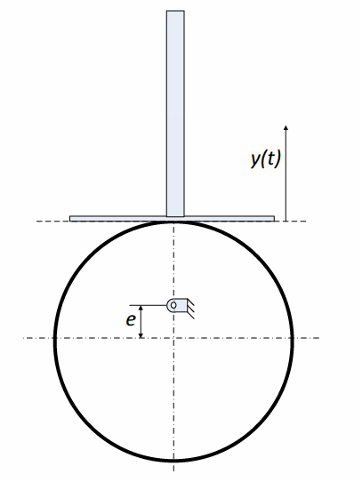
\includegraphics[width=0.4\textwidth]{Fig 3.png}
\caption{}
\label{fig:question5}
\end{figure}

\begin{multicols}{4}
\begin{enumerate}
    \item $ e \sin \omega t $
    \item $ e(1 + \cos 2\omega t) $
    \item $ e(1 - \cos \omega t) $
    \item $ e \sin 2\omega t $
\end{enumerate}
\end{multicols}
\hfill (GATE ME 2019)

\item The natural frequencies corresponding to the spring-mass systems I and II are $\omega_I$ and $\omega_{II}$, respectively. The ratio $\frac{\omega_I}{\omega_{II}}$ is

\begin{figure}[H]
\centering
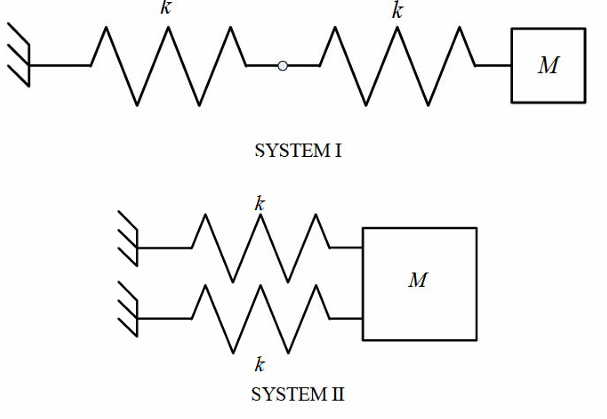
\includegraphics[width=0.8\textwidth]{Fig 4.png}
\caption{}
\label{fig:question6}
\end{figure}

\begin{multicols}{4}
\begin{enumerate}
    \item $\frac{1}{4}$
    \item $\frac{1}{2}$
    \item 2
    \item 4
\end{enumerate}
\end{multicols}
\hfill (GATE ME 2019)

\item A spur gear with $20^\circ$ full depth teeth is transmitting 20 kW at 200 rad/s. The pitch circle diameter of the gear is 100 mm. The magnitude of the force applied on the gear in the radial direction is
\begin{multicols}{4}
\begin{enumerate}
    \item 0.36 kN
    \item 0.73 kN
    \item 1.39 kN
    \item 2.78 kN
\end{enumerate}
\end{multicols}
\hfill (GATE ME 2019)

\item During a non-flow thermodynamic process (1-2) executed by a perfect gas, the heat interaction is equal to the work interaction ($Q_{1-2} = W_{1-2}$) when the process is
\begin{multicols}{2}
\begin{enumerate}
    \item Isentropic
    \item Polytropic
    \item Isothermal
    \item Adiabatic
\end{enumerate}
\end{multicols}
\hfill (GATE ME 2019)

\item For a hydrodynamically and thermally fully developed laminar flow through a circular pipe of constant cross-section, the Nusselt number at constant wall heat flux $ Nu_q $ and that at constant wall temperature $ Nu_T $ are related as
\begin{multicols}{2}
\begin{enumerate}
    \item $ Nu_q > Nu_T $
    \item $ Nu_q < Nu_T $
    \item $ Nu_q = Nu_T $
    \item $ Nu_q = (Nu_T)^2 $
\end{enumerate}
\end{multicols}
\hfill (GATE ME 2019)

\item As per common design practice, the three types of hydraulic turbines, in descending order of flow rate, are
\begin{enumerate}
    \item Kaplan, Francis, Pelton
    \item Pelton, Francis, Kaplan
    \item Francis, Kaplan, Pelton
    \item Pelton, Kaplan, Francis
\end{enumerate}
\hfill (GATE ME 2019)

\item A slender rod of length $ L $, diameter $ d $ ($ L >> d $) and thermal conductivity $ k_1 $ is joined with another rod of identical dimensions, but of thermal conductivity $ k_2 $, to form a composite cylindrical rod of length $ 2L $. The heat transfer in radial direction and contact resistance are negligible. The effective thermal conductivity of the composite rod is
\begin{multicols}{2}
\begin{enumerate}
    \item $ k_1 + k_2 $
    \item $ \sqrt{k_1 k_2} $
    \item $ \frac{k_1 k_2}{k_1 + k_2} $
    \item $ \frac{2k_1 k_2}{k_1 + k_2} $
\end{enumerate}
\end{multicols}
\hfill (GATE ME 2019)

\item Consider an ideal vapor compression refrigeration cycle. If the throttling process is replaced by an isentropic expansion process, keeping all the other processes unchanged, which one of the following statements is true for the modified cycle?
\begin{enumerate}
    \item Coefficient of performance is higher than that of the original cycle.
    \item Coefficient of performance is lower than that of the original cycle.
    \item Coefficient of performance is the same as that of the original cycle.
    \item Refrigerating effect is lower than that of the original cycle.
\end{enumerate}
\hfill (GATE ME 2019)

\item In a casting process, a vertical channel through which molten metal flows downward from pouring basin to runner for reaching the mold cavity is called
\begin{multicols}{4}
\begin{enumerate}
    \item blister
    \item sprue
    \item riser
    \item pin hole
\end{enumerate}
\end{multicols}
\hfill (GATE ME 2019)

\item Which one of the following welding methods provides the highest heat flux (W/mm²)?
\begin{multicols}{2}
\begin{enumerate}
    \item Oxy-acetylene gas welding
    \item Tungsten inert gas welding
    \item Plasma arc welding
    \item Laser beam welding
\end{enumerate}
\end{multicols}
\hfill (GATE ME 2019)

\item The length, width and thickness of a steel sample are 400 mm, 40 mm and 20 mm, respectively. Its thickness needs to be uniformly reduced by 2 mm in a single pass by using horizontal slab milling. The milling cutter (diameter: 100 mm, width: 50 mm) has 20 teeth and rotates at 1200 rpm. The feed per tooth is 0.05 mm. The feed direction is along the length of the sample. If the over-travel distance is the same as the approach distance, the approach distance and time taken to complete the required machining task are
\begin{multicols}{2}
\begin{enumerate}
    \item 14 mm, 18.4 s
    \item 21 mm, 28.9 s
    \item 21 mm, 39.4 s
    \item 14 mm, 21.4 s
\end{enumerate}
\end{multicols}
\hfill (GATE ME 2019)

\item The position vector $\overrightarrow{OP}$ of point $P(20, 10)$ is rotated anti-clockwise in the X–Y plane by an angle $\theta = 30^\circ$ such that point $P$ occupies position $Q$, as shown in the figure. The coordinates $(x, y)$ of $Q$ are:

\begin{figure}[H]
\centering
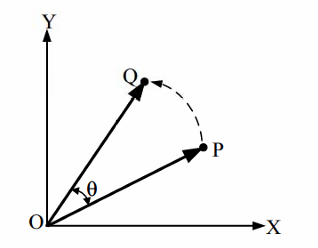
\includegraphics[width=0.5\textwidth]{Fig 5.png}
\caption{}
\label{fig:question16}
\end{figure}

\begin{multicols}{4}
\begin{enumerate}
\item (13.40, 22.32) 
\item (22.32, 8.26)  
\item (12.32, 18.66)  
\item (18.66, 12.32)  
\end{enumerate}
\end{multicols}
\hfill (GATE ME 2019)

\item The table presents the demand of a product. By simple three-months moving average method, the demand-forecast of the product for the month of September is:

\begin{center}
\begin{tabular}{|c|c|}
\hline
\textbf{Month} & \textbf{Demand} \\
\hline
January & 450 \\
\hline
February & 440 \\
\hline
March & 460 \\
\hline
April & 510 \\
\hline
May & 520 \\
\hline
June & 495 \\
\hline
July & 475 \\
\hline
August & 560 \\
\hline
\end{tabular}
\end{center}

\begin{multicols}{4}
\begin{enumerate}
\item 490
\item 510  
\item 530
\item 536.67  
\end{enumerate}
\end{multicols}

\hfill (GATE ME 2019)

\item Evaluation of $\int_{2}^{4} x^3 \, dx$ using a 2-equal-segment trapezoidal rule gives a value of -------------

\hfill (GATE ME 2019)

\item A block of mass 10 kg rests on a horizontal floor. The acceleration due to gravity is 9.81 m/s$^2$. The coefficient of static friction between the floor and the block is 0.2. A horizontal force of 10 N is applied on the block as shown in the figure. The magnitude of force of friction (in N) on the block is ----------

\begin{figure}[H]
\centering
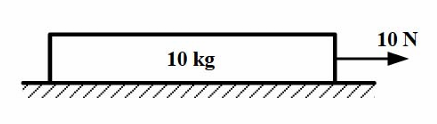
\includegraphics[width=0.3\textwidth]{Fig 6.png}
\caption{}
\label{fig:quetion19}
\end{figure}
\hfill (GATE ME 2019)

\item A cylindrical rod of diameter 10 mm and length 1.0 m is fixed at one end. The other end is twisted by an angle of 10° by applying a torque. If the maximum shear strain in the rod is $ p \times 10^{-3} $, then $ p $ is equal to ---------- (round off to two decimal places).
\hfill (GATE ME 2019)

\item A solid cube of side 1 m is kept at a room temperature of 32 \degree C. The coefficient of linear thermal expansion of the cube material is $ 1 \times 10^{-5} / \degree C $ and the bulk modulus is 200 GPa. If the cube is constrained all around and heated uniformly to 42 °C, then the magnitude of volumetric (mean) stress (in MPa) induced due to heating is ----------
\hfill (GATE ME 2019)

\item During a high cycle fatigue test, a metallic specimen is subjected to cyclic loading with a mean stress of +140 MPa, and a minimum stress of -70 MPa. The R-ratio (minimum stress to maximum stress) for this cyclic loading is ---------- (round off to one decimal place)
\hfill (GATE ME 2019)

\item Water flows through a pipe with a velocity given by $ \vec{V} = \left( \frac{4}{t} + x + y \right) \hat{y} $ m/s, where $ \hat{y} $ is the unit vector in the y direction, $ t > 0 $ is in seconds, and $ x $ and $ y $ are in meters. The magnitude of total acceleration at the point $ (x, y) = (1, 1) $ at $ t = 2 $ s is ---------- m/s$^2$.
\hfill (GATE ME 2019)

\item Air of mass 1 kg, initially at 300 K and 10 bar, is allowed to expand isothermally till it reaches a pressure of 1 bar. Assuming air as an ideal gas with gas constant of 0.287 kJ/kg.K, the change in entropy of air (in kJ/kg.K, round off to two decimal places) is ----------
\hfill (GATE ME 2019)

\item Consider the stress-strain curve for an ideal elastic-plastic strain hardening metal as shown in the figure. The metal was loaded in uniaxial tension starting from O. Upon loading, the stress-strain curve passes through initial yield point at P, and then strain hardens to point Q, where the loading was stopped. From point Q, the specimen was unloaded to point R, where the stress is zero. If the same specimen is reloaded in tension from point R, the value of stress at which the material yields again is ---------- MPa.

\begin{figure}[H]
\centering
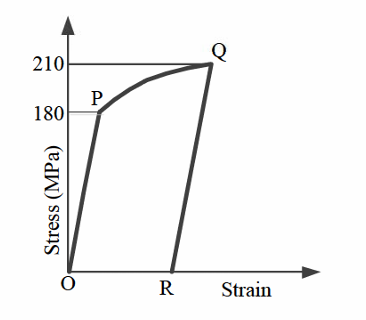
\includegraphics[width=0.5\textwidth]{Fig 7.png}
\caption{}
\label{fig:quetion25}
\end{figure}
\hfill (GATE ME 2019)


\textbf{Q. 26 – Q. 55 carry two marks each.}


\item The set of equations
$\begin{aligned}
x + y + z &= 1 \\
ax - ay + 3z &= 5 \\
5x - 3y + az &= 6
\end{aligned}$
has infinite solutions, if $ a = $
\begin{multicols}{4}
\begin{enumerate}
    \item -3
    \item 3
    \item 4
    \item -4
\end{enumerate}
\end{multicols}
\hfill (GATE ME 2019)

\item A harmonic function is analytic if it satisfies the Laplace equation.
If $ u(x,y) = 2x^2 - 2y^2 + 4xy $ is a harmonic function, then its conjugate harmonic function $ v(x,y) $ is
\begin{enumerate}
    \item $ 4xy - 2x^2 + 2y^2 + $ constant
    \item $ 4y^2 - 4xy + $ constant
    \item $ 2x^2 - 2y^2 + xy + $ constant
    \item $ -4xy + 2y^2 - 2x^2 + $ constant
\end{enumerate}
\hfill (GATE ME 2019)

\item The variable $ x $ takes a value between 0 and 10 with uniform probability distribution. The variable $ y $ takes a value between 0 and 20 with uniform probability distribution. The probability of the sum of variables $ (x + y) $ being greater than 20 is
\begin{multicols}{4}
\begin{enumerate}
    \item 0
    \item 0.25
    \item 0.33
    \item 0.50
\end{enumerate}
\end{multicols}
\hfill (GATE ME 2019)

\item A car having weight \textit{W} is moving in the direction as shown in the figure. The center of gravity (CG) of the car is located at height \textit{h} from the ground, midway between the front and rear wheels. The distance between the front and rear wheels \textit{l}. The acceleration of the car is \textit{a}, and acceleration due to gravity is \textit{g}. The reactions on the front wheels $(R_f)$ and rear wheels $(R_f)$ are given by
\begin{figure}[H]
\centering
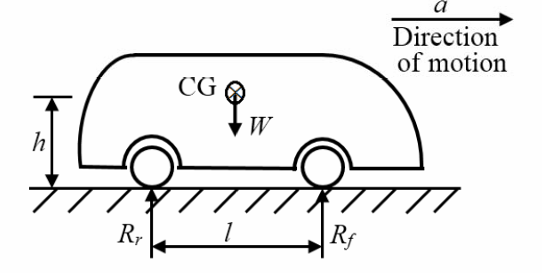
\includegraphics[width=0.8\textwidth]{Fig 8.png}
\caption{}
\label{fig:question29}
\end{figure}
\begin{enumerate}
\item $ R_f = R_r = \frac{W}{2} - \frac{W}{g} \left( \frac{h}{l} \right) a $ 
\item $ R_f = \frac{W}{2} + \frac{W}{g} \left( \frac{h}{l} \right) a ;\quad R_r = \frac{W}{2} - \frac{W}{g} \left( \frac{h}{l} \right) a $ 
\item $ R_f = \frac{W}{2} - \frac{W}{g} \left( \frac{h}{l} \right) a ;\quad R_r = \frac{W}{2} + \frac{W}{g} \left( \frac{h}{l} \right) a $ 
\item $ R_f = R_r = \frac{W}{2} + \frac{W}{g} \left( \frac{h}{l} \right) a $ 
\end{enumerate}
\hfill (GATE ME 2019)

\item In a four-bar planar mechanism shown in the figure, $ AB = 5\, \text{cm} $, $ AD = 4\, \text{cm} $, and $ DC = 2\, \text{cm} $. In the configuration shown, both $ AB $ and $ DC $ are perpendicular to $ AD $. The bar $ AB $ rotates with an angular velocity of $ 10\, \text{rad/s} $. The magnitude of angular velocity (in rad/s) of bar $ DC $ at this instant is:

\begin{figure}[H]
\centering
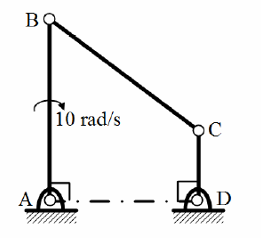
\includegraphics[width=0.5\textwidth]{Fig 9.png}
\caption{}
\label{fig:question30}
\end{figure}

\begin{multicols}{4}
\begin{enumerate}
\item 0  
\item 10  
\item 15  
\item 25  
\end{enumerate}
\end{multicols}
\hfill (GATE ME 2019)

\item The rotor of a turbojet engine of an aircraft has a mass 180 kg and polar moment of inertia 10 kg·m$^2$ about the rotor axis. The rotor rotates at a constant speed of 1100 rad/s in the clockwise direction when viewed from the front of the aircraft. The aircraft while flying at a speed of 800 km per hour takes a turn with a radius of 1.5 km to the left. The gyroscopic moment exerted by the rotor on the aircraft structure and the direction of motion of the nose when the aircraft turns, are
\begin{enumerate}
\item 1629.6 N·m and the nose goes up
\item 1629.6 N·m and the nose goes down
\item 162.9 N·m and the nose goes up
\item 162.9 N·m and the nose goes down
\end{enumerate}
\hfill (GATE ME 2019)

\item The wall of a constant diameter pipe of length 1 m is heated uniformly with flux $ q'' $ by wrapping a heater coil around it. The flow at the inlet to the pipe is hydrodynamically fully developed. The fluid is incompressible and the flow is assumed to be laminar and steady all through the pipe. The bulk temperature of the fluid is equal to 0°C at the inlet and 50°C at the exit. The wall temperatures are measured at three locations, P, Q and R, as shown in the figure. The flow thermally develops after some distance from the inlet. The following measurements are made:

\begin{tabular}{|c|c|c|c|}
\hline
Point & P & Q & R \\
\hline
Wall Temp (°C) & 50 & 80 & 90 \\
\hline
\end{tabular}

\begin{figure}[H]
\centering
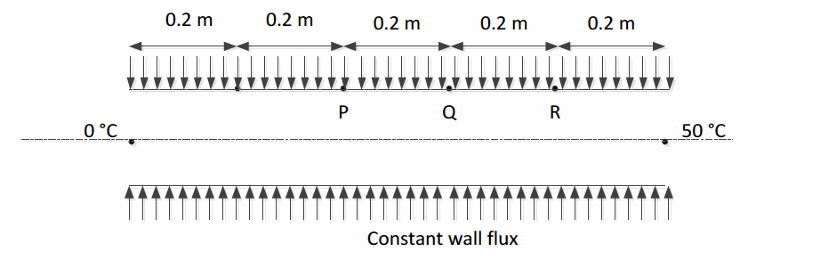
\includegraphics[width=0.8\textwidth]{Fig 10.png}
\caption{}
\label{fig:question32}
\end{figure}

Among the locations P, Q and R, the flow is thermally developed at
\begin{multicols}{4}
\begin{enumerate}
    \item P, Q and R
    \item P and Q only
    \item Q and R only
    \item R only
\end{enumerate}
\end{multicols}
\hfill (GATE ME 2019)

\item A gas is heated in a duct as it flows over a resistance heater. Consider a 101 kW electric heating system. The gas enters the heating section of the duct at 100 kPa and 27 °C with a volume flow rate of 15 m$^3$/s. If heat is lost from the gas in the duct to the surroundings at a rate of 51 kW, the exit temperature of the gas is

(Assume constant pressure, ideal gas, negligible change in kinetic and potential energies and constant specific heat; $ C_p = 1 \, \text{kJ/kg·K} $; $ R = 0.5 \, \text{kJ/kg·K} $)
\begin{multicols}{4}
\begin{enumerate}
    \item 32 °C
    \item 37 °C
    \item 53 °C
    \item 76 °C
\end{enumerate}
\end{multicols}
\hfill (GATE ME 2019)

\item A plane-strain compression (forging) of a block is shown in the figure. The strain in the z-direction is zero. The yield strength ($ S_y $) in uniaxial tension/compression of the material of the block is 300 MPa and it follows the Tresca (maximum shear stress) criterion. Assume that the entire block has started yielding. At a point where $ \sigma_x = 40 \, \text{MPa} $ (compressive) and $ \tau_{xy} = 0 $, the stress component $ \sigma_y $ is

\begin{figure}[H]
\centering
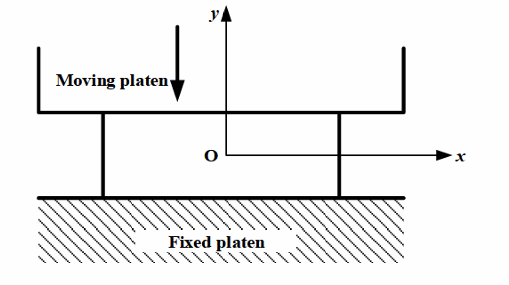
\includegraphics[width=0.5\textwidth]{Fig 11.png}
\caption{}
\label{fig:question34}
\end{figure}

\begin{multicols}{2}
\begin{enumerate}
    \item 340 MPa (compressive)
    \item 340 MPa (tensile)
    \item 260 MPa (compressive)
    \item 260 MPa (tensile)
\end{enumerate}
\end{multicols}
\hfill (GATE ME 2019)

\item In orthogonal turning of a cylindrical tube of wall thickness 5 mm, the axial and the tangential cutting forces were measured as 1259 N and 1601 N, respectively. The measured chip thickness after machining was found to be 0.3 mm. The rake angle was 10° and the axial feed was 100 mm/min. The rotational speed of the spindle was 1000 rpm. Assuming the material to be perfectly plastic and Merchant's first solution, the shear strength of the material is closest to
\begin{multicols}{4}
\begin{enumerate}
    \item 722 MPa
    \item 920 MPa
    \item 200 MPa
    \item 875 MPa
\end{enumerate}
\end{multicols}
\hfill (GATE ME 2019)

\item A circular shaft having diameter 65.00±0.01±0.05 mm is manufactured by turning process. A 50 $\mu$m thick coating of TiN is deposited on the shaft. Allowed variation in TiN film thickness is ± 5 $\mu$m. The minimum hole diameter (in mm) to just provide clearance fit is
\begin{multicols}{4}
\begin{enumerate}
    \item 65.01
    \item 65.12
    \item 64.95
    \item 65.10
\end{enumerate}
\end{multicols}
\hfill (GATE ME 2019)

\item Match the following sand mold casting defects with their respective causes.

\begin{tabular}{|c|c|}
\hline
Defect & Cause \\
\hline
P   Blow hole & 1 Poor collapsibility \\
\hline
Q   Misrun & 2 Mold erosion \\
\hline
R   Hot tearing & 3 Poor permeability \\
\hline
S   Wash & 4 Insufficient fluidity \\
\hline
\end{tabular}

\begin{multicols}{2}
\begin{enumerate}
    \item P-4, Q-3, R-1, S-2
    \item P-3, Q-4, R-2, S-1
    \item P-2, Q-4, R-1, S-3
    \item P-3, Q-4, R-1, S-2
\end{enumerate}
\end{multicols}
\hfill (GATE ME 2019)

\item A truss is composed of members AB, BC, CD, AD and BD, as shown in the figure. A vertical load of 10 kN is applied at point D. The magnitude of force (in kN) in the member BC is ----------

\begin{figure}[H]
\centering
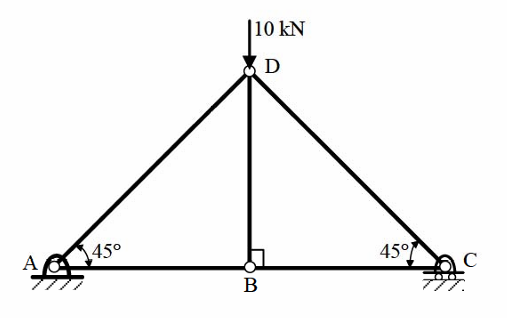
\includegraphics[width=0.5\textwidth]{Fig 12.png}
\caption{}
\label{fig:question38}
\end{figure}
\hfill (GATE ME 2019)

\item Consider an elastic straight beam of length $ L = 10 \pi $ m, with square cross-section of side $ \alpha = 5 $ mm, and Young's modulus $ E = 200 $ GPa. This straight beam was bent in such a way that the two ends meet, to form a circle of mean radius $ R $. Assuming that Euler-Bernoulli beam theory is applicable to this bending problem, the maximum tensile bending stress in the bent beam is ---------- MPa.

\begin{figure}[H]
\centering
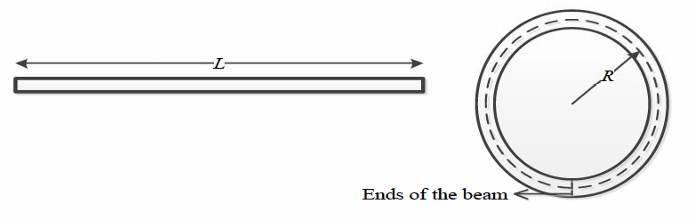
\includegraphics[width=0.8\textwidth]{Fig 13.png}
\caption{}
\label{fig:question39}
\end{figure}
\hfill (GATE ME 2019)

\item Consider a prismatic straight beam of length $ L = \pi $ m, pinned at the two ends as shown in the figure. The beam has a square cross-section of side $ p = 6 $ mm. The Young's modulus $ E = 200 $ GPa, and the coefficient of thermal expansion $ \alpha = 3 \times 10^{-6} \, \text{K}^{-1} $. The minimum temperature rise required to cause Euler buckling of the beam is ---------- K.

\begin{figure}[H]
\centering
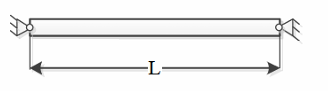
\includegraphics[width=0.4\textwidth]{Fig 14.png}
\caption{}
\label{fig:question40}
\end{figure}
\hfill (GATE ME 2019)

\item In a UTM experiment, a sample of length 100 mm, was loaded in tension until failure. The failure load was 40 kN. The displacement, measured using the cross-head motion, at failure, was 15 mm. The compliance of the UTM is constant and is given by $ 5 \times 10^{-8} $ m/N. The strain at failure in the sample is ----------\%.

\hfill (GATE ME 2019)

\item At a critical point in a component, the state of stress is given as $ \sigma_{xx} = 100 \, \text{MPa} $, $ \sigma_{yy} = 220 \, \text{MPa} $, $ \sigma_{xy} = \sigma_{yx} = 80 \, \text{MPa} $ and all other stress components are zero. The yield strength of the material is 468 MPa. The factor of safety on the basis of maximum shear stress theory is ---------- (round off to one decimal place).

\hfill (GATE ME 2019)

\item A uniform thin disk of mass 1 kg and radius 0.1 m is kept on a surface as shown in the figure. A spring of stiffness $ k_1 = 400 \, \text{N/m} $ is connected to the disk center A and another spring of stiffness $ k_2 = 100 \, \text{N/m} $ is connected at point B just above point A on the circumference of the disk. Initially, both the springs are unstretched. Assume pure rolling of the disk. For small disturbance from the equilibrium, the natural frequency of vibration of the system is ---------- rad/s (round off to one decimal place).

\begin{figure}[H]
\centering
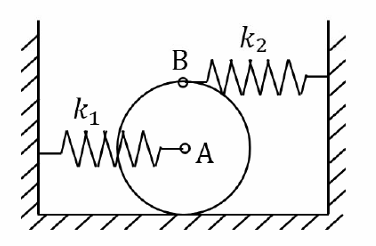
\includegraphics[width=0.5\textwidth]{Fig 15.png}
\caption{}
\label{fig:question43}
\end{figure}
\hfill (GATE ME 2019)

\item A single block brake with a short shoe and torque capacity of 250 N·m is shown. The cylindrical brake drum rotates anticlockwise at 100 rpm and the coefficient of friction is 0.25. The value of $ a $, in mm (round off to one decimal place), such that the maximum actuating force $ P $ is 2000 N, is ----------.

\begin{figure}[H]
\centering
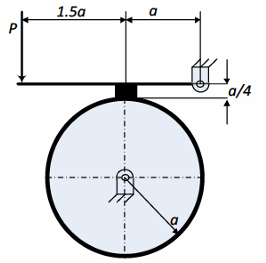
\includegraphics[width=0.5\textwidth]{Fig 16.png}
\caption{}
\label{fig:question44}
\end{figure}
\hfill (GATE ME 2019)

\item Two immiscible, incompressible, viscous fluids having same densities but different viscosities are contained between two infinite horizontal parallel plates, 2 m apart as shown below. The bottom plate is fixed and the upper plate moves to the right with a constant velocity of 3 m/s. With the assumptions of Newtonian fluid, steady, and fully developed laminar flow with zero pressure gradient in all directions, the momentum equations simplify to
$\frac{d^2 u}{dy^2} = 0.$

If the dynamic viscosity of the lower fluid, $\mu_2$, is twice that of the upper fluid, $\mu_1$, then the velocity at the interface (round off to two decimal places) is ---------- m/s.

\begin{figure}[H]
\centering
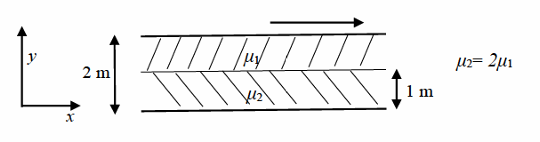
\includegraphics[width=0.6\textwidth]{Fig 17.png}
\caption{}
\label{fig:question45}
\end{figure}
\hfill (GATE ME 2019)

\item A cube of side 100 mm is placed at the bottom of an empty container on one of its faces. The density of the material of the cube is 800 kg/m$^3$. Liquid of density 1000 kg/m$^3$ is now poured into the container. The minimum height to which the liquid needs to be poured into the container for the cube to just lift up is ---------- mm.

\hfill (GATE ME 2019)

\item Three slabs are joined together as shown in the figure. There is no thermal contact resistance at the interfaces. The center slab experiences a non-uniform internal heat generation with an average value equal to 10000 Wm$^{-3}$, while the left and right slabs have no internal heat generation. All slabs have thickness equal to 1 m and thermal conductivity of each slab is equal to 5 Wm$^{-1}$K$^{-1}$. The two extreme faces are exposed to fluid with heat transfer coefficient 100 Wm$^{-2}$K$^{-1}$ and bulk temperature 30 °C as shown. The heat transfer in the slabs is assumed to be one dimensional and steady, and all properties are constant. If the left extreme face temperature $ T_1 $ is measured to be 100 °C, the right extreme face temperature $ T_2 $ is ----------°C.

\begin{figure}[H]
\centering
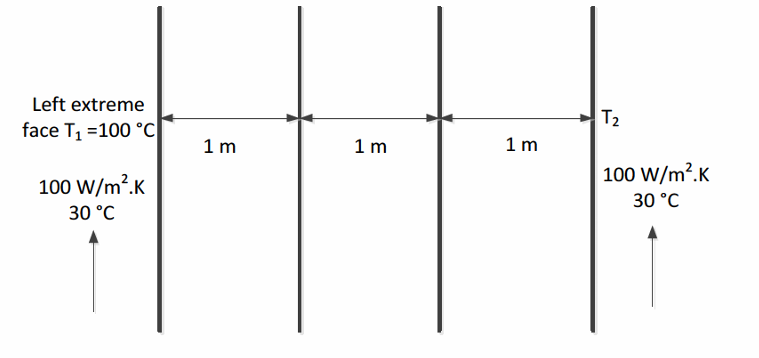
\includegraphics[width=0.8\textwidth]{Fig 18.png}
\caption{}
\label{fig:question47}
\end{figure}
\hfill (GATE ME 2019)

\item If one mole of $ H_2 $ gas occupies a rigid container with a capacity of 1000 litres and the temperature is raised from 27 °C to 37 °C, the change in pressure of the contained gas (round off to two decimal places), assuming ideal gas behaviour, is ---------- Pa. ($ R = 8.314 \, \text{J/mol·K} $)

\hfill (GATE ME 2019)

\item A steam power cycle with regeneration as shown below on the $ T $-$ s $ diagram employs a single open feedwater heater for efficiency improvement. The fluids mix with each other in an open feedwater heater. The turbine is isentropic and the input (bleed) to the feedwater heater from the turbine is at state 2 as shown in the figure. Process 3-4 occurs in the condenser. The pump work is negligible. The input to the boiler is at state 5. The following information is available from the steam tables:

\begin{tabular}{|c|c|c|c|c|c|c|}
\hline
State & 1 & 2 & 3 & 4 & 5 & 6 \\
\hline
Enthalpy (kJ/kg) & 3350 & 2800 & 2300 & 175 & 700 & 1000 \\
\hline
\end{tabular}

\begin{figure}[H]
\centering
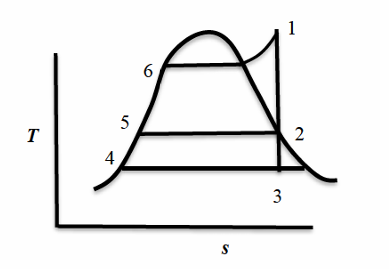
\includegraphics[width=0.5\textwidth]{Fig 19.png}
\caption{}
\label{fig:question49}
\end{figure}
The mass flow rate of steam bled from the turbine as a percentage of the total mass flow rate at the inlet to the turbine at state 1 is ----------

\hfill (GATE ME 2019)

\item A gas turbine with air as the working fluid has an isentropic efficiency of 0.70 when operating at a pressure ratio of 3. Now, the pressure ratio of the turbine is increased to 5, while maintaining the same inlet conditions. Assume air as a perfect gas with specific heat ratio $\gamma = 1.4$. If the specific work output remains the same for both the cases, the isentropic efficiency of the turbine at the pressure ratio of 5 is ---------- (round off to two decimal places)

\hfill (GATE ME 2019)

\item The value of the following definite integral is ---------- (round off to three decimal places)

\begin{center}
$\int_{1}^{e} (x \ln x) dx$
\end{center}

\hfill (GATE ME 2019)

\item In ASA system, the side cutting and end cutting edge angles of a sharp turning tool are 45° and 10°, respectively. The feed during cylindrical turning is 0.1 mm/rev. The center line average surface roughness (in µm, round off to one decimal place) of the generated surface is ----------

\hfill (GATE ME 2019)

\item Taylor's tool life equation is given by $ VT^n = C $, where $ V $ is in m/min and $ T $ is in min. In a turning operation, two tools X and Y are used. For tool X, $ n = 0.3 $ and $ C = 60 $ and for tool Y, $ n = 0.6 $ and $ C = 90 $. Both the tools will have the same tool life for the cutting speed (in m/min, round off to one decimal place) of ----------

\hfill (GATE ME 2019)

\item Five jobs (J1, J2, J3, J4 and J5) need to be processed in a factory. Each job can be assigned to any of the five different machines (M1, M2, M3, M4 and M5). The time durations taken (in minutes) by the machines for each of the jobs, are given in the table. However, each job is assigned to a specific machine in such a way that the total processing time is minimum. The total processing time is ---------- minutes.

\begin{tabular}{|c|c|c|c|c|c|}
\hline
 & M1 & M2 & M3 & M4 & M5 \\
\hline
J1 & 40 & 30 & 50 & 50 & 58 \\
\hline
J2 & 26 & 38 & 60 & 26 & 38 \\
\hline
J3 & 40 & 34 & 28 & 24 & 30 \\
\hline
J4 & 28 & 40 & 40 & 32 & 48 \\
\hline
J5 & 28 & 32 & 38 & 22 & 44 \\
\hline
\end{tabular}

\hfill (GATE ME 2019)

\item A project consists of six activities. The immediate predecessor of each activity and the estimated duration is also provided in the table below:

\begin{tabular}{|c|c|c|}
\hline
Activity & Immediate predecessor & Estimated duration (weeks) \\
\hline
P & - & 5 \\
\hline
Q & - & 1 \\
\hline
R & Q & 2 \\
\hline
S & P, R & 4 \\
\hline
T & P & 6 \\
\hline
U & S, T & 3 \\
\hline
\end{tabular}

If all activities other than S take the estimated amount of time, the maximum duration (in weeks) of the activity S without delaying the completion of the project is ----------

\hfill (GATE ME 2019)


\end{enumerate}
\end{document}